% Hai section thay thế: diff.c và du.c
% Giữ các macro \code{} của báo cáo gốc.
% Preamble cần: \usepackage{graphicx}, \usepackage{float}, \usepackage{enumitem}.

\section{diff.c}

\subsection{Tổng quan}
\texttt{diff.c} được xây dựng nhằm so sánh hai tệp văn bản theo từng dòng và thông báo
những vị trí có nội dung khác nhau. Chương trình tham khảo chức năng của
\texttt{diff} trên Unix và quy ước mã thoát được quy định trong đặc tả POSIX
\cite{posix2018diff}. Tuy nhiên, thay vì tìm một tập phép thêm, xóa hoặc thay đổi
dòng để biến đổi tệp thứ nhất thành tệp thứ hai như \texttt{diff} tiêu chuẩn, phiên bản
của nhóm so sánh trực tiếp các dòng ở cùng vị trí. Vì vậy, đầu ra phản ánh sự khác biệt
theo chỉ số dòng, không phải một bản mô tả chỉnh sửa tối thiểu như các thuật toán so
sánh tệp truyền thống \cite{hunt1976algorithm}.

Trong xv6, thư viện người dùng chỉ cung cấp một tập hàm tương đối hạn chế, không có sẵn
các hàm đọc dòng như \texttt{getline()} hay \texttt{fgets()} \cite{xv6book}. Do đó, nhóm
xây dựng hàm \code{readline()} để đọc dữ liệu từ file descriptor bằng \code{read()},
đồng thời quản lý bộ đệm động và trạng thái ký tự xuống dòng.

\begin{figure}[H]
    \centering
    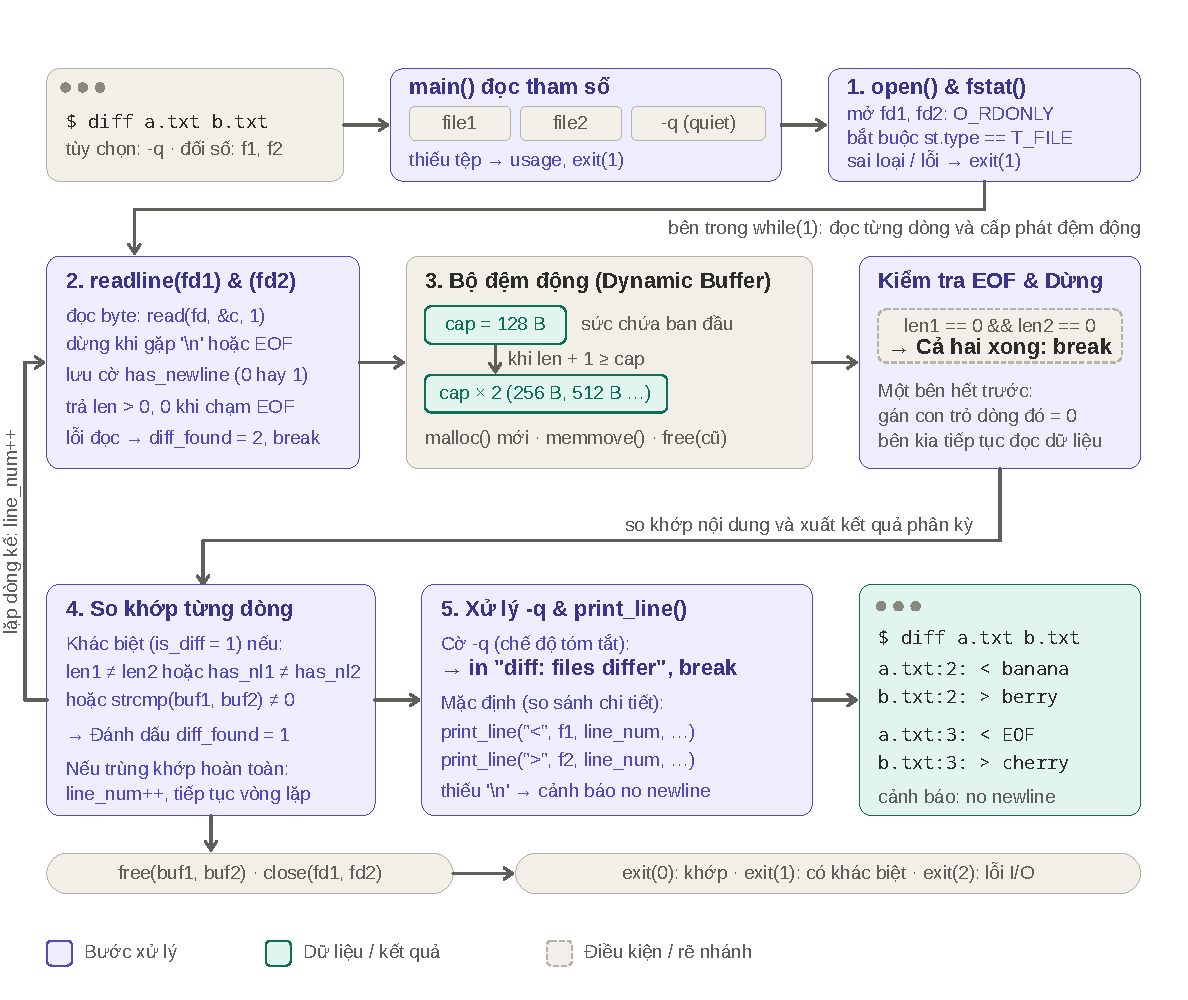
\includegraphics[width=0.52\textwidth]{images/diff_workflow.pdf}
    \caption{Sơ đồ luồng thực thi và cơ chế so sánh dòng trong \texttt{diff.c}}
    \label{fig:diff_workflow}
\end{figure}

\noindent Luồng thực thi gồm các giai đoạn:
\begin{itemize}[noitemsep, topsep=2pt]
    \item \textbf{Mở và kiểm tra tệp:} Phân tích tham số dòng lệnh, mở hai tệp với cờ
        \code{O\_RDONLY}, sau đó dùng \code{fstat()} để xác nhận cả hai là tệp thường
        (\code{st.type == T\_FILE}), tránh xử lý nhầm thư mục hoặc thiết bị.
    \item \textbf{Đọc từng dòng:} Hàm \code{readline()} sử dụng hai bộ đệm độc lập, mỗi
        bộ đệm có dung lượng ban đầu 128 byte. Khi một dòng dài hơn sức chứa hiện tại,
        chương trình cấp phát vùng nhớ mới với dung lượng gấp đôi, sao chép dữ liệu bằng
        \code{memmove()} và giải phóng vùng nhớ cũ.
    \item \textbf{So sánh và xuất kết quả:} Với mỗi cặp dòng cùng chỉ số, chương trình
        đối chiếu chiều dài, cờ \code{has\_newline} và nội dung bằng \code{strcmp()}.
        Khi phát hiện khác biệt, hàm \code{print\_line()} hiển thị dòng tương ứng của
        từng tệp với tiền tố \code{<} và \code{>} cùng số dòng để người dùng xác định vị
        trí sai khác.
\end{itemize}

\subsection{Khó khăn và Thử thách}
Trong quá trình triển khai, nhóm tập trung xử lý các trường hợp biên liên quan đến việc
đọc dòng và quản lý tài nguyên trên xv6:

\begin{enumerate}[noitemsep, topsep=2pt]
    \item \textbf{Hai tệp có số dòng khác nhau:}
    Khi một tệp kết thúc trước tệp còn lại, chương trình phải phân biệt được trạng thái
    hết tệp (EOF) với một dòng rỗng hợp lệ. Nếu chỉ dựa vào độ dài nội dung bằng 0, việc
    so sánh có thể dừng sớm hoặc bỏ sót những dòng còn lại. \\
    \textit{Giải pháp:} Nhóm xử lý riêng trạng thái kết thúc của từng luồng đọc. Hàm
    \code{print\_line()} cho phép biểu diễn phía đã hết tệp bằng \code{EOF}, đồng thời
    tiếp tục đọc và hiển thị những dòng còn lại ở phía kia cho đến khi cả hai luồng đều
    kết thúc. Cách xử lý này bảo toàn thông tin về các dòng dư, dù không tự động căn
    chỉnh những đoạn văn bản bị thêm hoặc xóa ở giữa tệp.

    \item \textbf{Dòng cuối không có ký tự xuống dòng:}
    Hai dòng có cùng chuỗi ký tự nhưng khác nhau về việc có kết thúc bằng
    \code{'\textbackslash n'} hay không không nên bị xem là hoàn toàn giống nhau. Đây là
    một trường hợp cần lưu ý khi so sánh tệp văn bản theo dòng \cite{posix2018diff}. \\
    \textit{Giải pháp:} Hàm \code{readline()} lưu cờ \code{has\_newline} cho mỗi dòng và
    đưa cờ này vào điều kiện so sánh. Nếu dòng cuối không có ký tự xuống dòng, chương
    trình chủ động xuống dòng khi xuất kết quả và thông báo \texttt{no newline at end of
    file} để phân biệt hai trường hợp.

    \item \textbf{Chế độ so sánh nhanh và mã thoát:}
    Khi chỉ cần biết hai tệp có khác nhau hay không, việc in toàn bộ các dòng sai khác
    gây ra I/O không cần thiết. Tùy chọn \code{-q} được tham khảo từ chế độ
    \textit{brief} của GNU Diffutils \cite{gnudiffmanual}. \\
    \textit{Giải pháp:} Khi bật \code{-q}, chương trình dừng ở khác biệt đầu tiên, đặt
    \code{is\_diff = 1} và in thông báo \texttt{diff: files differ}. Trước khi thoát,
    chương trình đóng các file descriptor và giải phóng bộ đệm đã cấp phát. Mã thoát
    được quy ước là \code{0} nếu hai tệp giống nhau, \code{1} nếu có khác biệt và
    \code{2} nếu xảy ra lỗi, tương thích với quy ước của \texttt{diff} trong POSIX
    \cite{posix2018diff}.
\end{enumerate}

\section{du.c}

\subsection{Tổng quan}
\texttt{du.c} (\textit{Disk Usage}) mô phỏng tiện ích cốt lõi trên các hệ điều hành họ Unix theo chuẩn POSIX \cite{posix2018du}, hỗ trợ ước tính dung lượng chiếm dụng của cây thư mục và tập tin bằng thuật toán duyệt đệ quy hậu thứ tự (\textit{post-order bottom-up traversal}). Tổng dung lượng của một thư mục được định nghĩa bằng tổng dung lượng thực tế của tất cả các tệp tin và cây con bên trong nó.

Trong hệ thống tệp xv6 \cite{xv6book}, một thư mục được tổ chức như một tập tin đặc biệt chứa danh sách các bản ghi \texttt{struct dirent} ($16\text{ bytes}$ gồm $2\text{ bytes}$ chỉ mục \texttt{inum} và $14\text{ bytes}$ tên \texttt{name}). Kích thước byte thực tế \texttt{st.size} của từng inode được truy xuất chính xác thông qua lời gọi hệ thống \code{stat()}.

\begin{figure}[H]
    \centering
    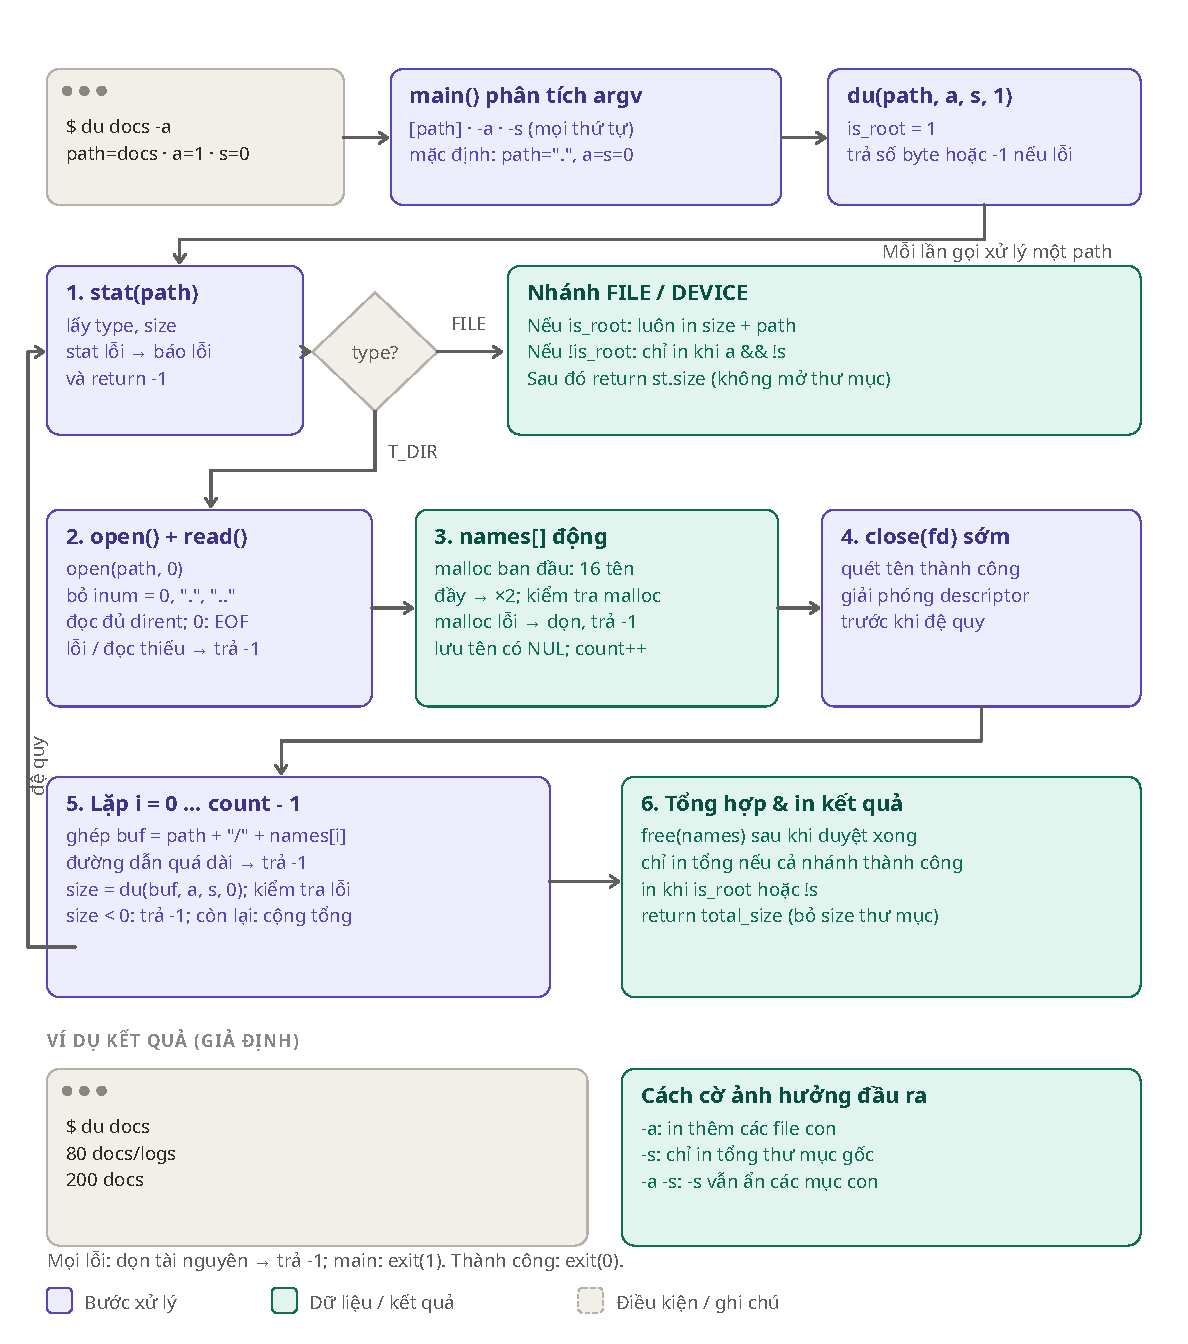
\includegraphics[width=0.70\textwidth]{images/du_workflow.pdf}
    \caption{Sơ đồ luồng thực thi duyệt đệ quy Bottom-up và giải phóng FD sớm trong \texttt{du.c}}
    \label{fig:du_workflow}
\end{figure}

\noindent Luồng thực thi diễn ra tuần tự qua các giai đoạn:
\begin{itemize}[noitemsep, topsep=2pt]
    \item \textbf{Khởi tạo và phân tích đối số:} Tiếp nhận đường dẫn mục tiêu (mặc định là \code{"."}), phân tích cờ tóm tắt \code{-s} (chỉ in kích thước thư mục gốc) và cờ chi tiết \code{-a} (in toàn bộ kích thước tệp tin đơn lẻ lẫn thư mục con).
    \item \textbf{Điều kiện dừng (Base Case):} Sử dụng \code{stat(path, \&st)}. Nếu đường dẫn trỏ tới một tệp tin thường (\code{T\_FILE}) hoặc tệp thiết bị (\code{T\_DEVICE}), kích thước \code{st.size} được trả về ngay lập tức; đồng thời in thông tin ra màn hình nếu đường dẫn là gốc được chỉ định hoặc có cờ \code{-a} (\code{is\_root || (a \&\& !s)}).
    \item \textbf{Duyệt con và cộng dồn (Bottom-up):} Khi gặp thư mục (\code{T\_DIR}), chương trình quét nội dung thư mục, lưu danh sách các tên tệp con hợp lệ, tiến hành gọi đệ quy \code{du(buf, a, s, 0)} cho từng nhánh con và cộng dồn vào biến \code{total\_size}. Thư mục hoàn thành đệ quy sẽ in kích thước tích lũy của chính nó trước khi trả kết quả về cho thư mục cha.
\end{itemize}

\subsection{Khó khăn và Thử thách}
Dựa trên kiến trúc của hệ điều hành xv6 và các ca biên trong quản lý tệp tin \cite{xv6book}, nhóm nhận thấy các khó khăn như sau:

\begin{enumerate}[noitemsep, topsep=2pt]
    \item \textbf{Giới hạn File Descriptor (\code{NOFILE = 16}):}
    Trong kernel xv6, mỗi tiến trình bị giới hạn mở tối đa 16 file descriptors đồng thời (\code{NOFILE = 16} trong \texttt{kernel/param.h}) \cite{xv6book}. Nếu duy trì \code{fd} của thư mục đang mở trong suốt các lời gọi đệ quy sâu, hệ thống sẽ nhanh chóng cạn kiệt FD khi độ sâu thư mục vượt quá ngưỡng cho phép, gây lỗi sập chương trình. \\
    \textit{Giải pháp:} Đọc toàn bộ tên các mục con vào mảng động \code{names} trên bộ nhớ heap, sau đó thực hiện lệnh \code{close(fd)} ngay lập tức trước khi bắt đầu bất kỳ lời gọi đệ quy con nào. Kỹ thuật này giúp số lượng FD mở tại mỗi thời điểm chỉ là $O(1)$ (tối đa 1 FD trong lúc đọc), bảo đảm an toàn với mọi độ sâu cấu trúc thư mục.

    \item \textbf{Phòng chống lặp vô hạn và lọc Inode rác:}
    Mọi thư mục Unix đều chứa hai thực thể liên kết cứng đặc thù là \texttt{"."} (thư mục hiện hành) và \texttt{".."} (thư mục cha). Ngoài ra, các entry đã xóa trong xv6 vẫn tồn tại trong bảng chỉ mục với \code{inum == 0}. \\
    \textit{Giải pháp:} Chủ động loại bỏ các khối có \code{de.inum == 0} và kiểm tra lọc bỏ chuỗi \texttt{"."} cùng \texttt{".."}, tránh hoàn toàn nguy cơ lặp đệ quy vô hạn làm tràn stack kernel và đảm bảo tính chính xác của phép cộng dồn dung lượng.

    \item \textbf{Quản lý bộ nhớ mảng động và kiểm soát đường dẫn:}
    Số lượng phần tử trong một thư mục là biến thiên và không thể biết trước, trong khi việc ghép nối chuỗi đường dẫn đệ quy tiềm ẩn nguy cơ tràn mảng đệm. \\
    \textit{Giải pháp:} Khởi tạo mảng con trỏ \code{names} ban đầu với sức chứa 16 phần tử, tự động tăng gấp đôi kích thước (\code{capacity * 2}) qua \code{malloc()} và \code{memmove()} khi danh sách vượt ngưỡng. Đồng thời, trước khi ghép chuỗi đường dẫn con, chương trình luôn kiểm tra điều kiện an toàn: \code{strlen(path) + 1 + strlen(names[i]) < sizeof(buf)} và giải phóng vùng nhớ sau khi sử dụng.
\end{enumerate}